\section{Motivating Scenario}
\label{sec:motivatingscenario}

IT industries aim to reduce their budget in expensive hardware investment and maintenance, e.g. Database Management Systems, while maintaining data access and persistency over time. In order to fulfill a budget reduction while maintaining their data and database system requirements, the data can be migrated to different Cloud storage providers available nowadays in the market. Considering the application's migrations types discussed in \cite{andrikopoulos2013}, migrating local data to the Cloud, and then accessing it from the application's hosted on-premise, can be considered as a \term{partial or complete replacement of components with Cloud offerings}. Such migration requires a reconfiguration, rewiring, and adaptation activities on both the migrated and non-migrated components.

The \term{Cloud Data Migration Application} assists the user in the migrating decision and process of local data to a Cloud storage provider, or from two different Cloud storage providers \cite{bachmann2012}. It contains a registry of the different available Cloud data stores, e.g. Amazon Dynamo DB  \cite{amazondynamodb}, Amazon RDS \cite{amazonrds}, Google Cloud SQL \cite{googlecloudsql}, and detects possible incompatibilities between the source and target data sources prior to the migration process.

Migration of data can be either seen as the migration of only the Data Layer, or as a part of the migration of the whole application \cite{andrikopoulos2013}. The approach we consider as the start point in this diploma thesis is the migration of the Data Layer, which contains two sublayers: the \term{Database Layer (DBL)} and the \term{Data Access Layer (DAL)}. The DBL contains the database information, e.g. location, access credentials, etc., and gives the DAL a direct communication support to the database server. The DAL provides simplified access support to the upper layers of the data stored in a backend database. However, migrating the Data Layer to the Cloud implies adaptations and rewiring of the original application. One of our main goals in this diploma thesis is to minimize the needed adaptations in the non-migrated and migrated components by providing a transparent access to the user's data migrated to a Cloud datastore. 

As the Enterprise Service Bus is an established integration middleware for services in Service-Oriented Architectures (SOA), and due to its multi-protocol support and reliable internal messaging routing, we use it as a central piece for providing a multi-tenant aware, transparent and reliable communication support between the on-premise and the off-premise layers of the application.

%\cite{4CaaSt} \ac{HTTP}

\begin{figure}[htb]
	\centering
		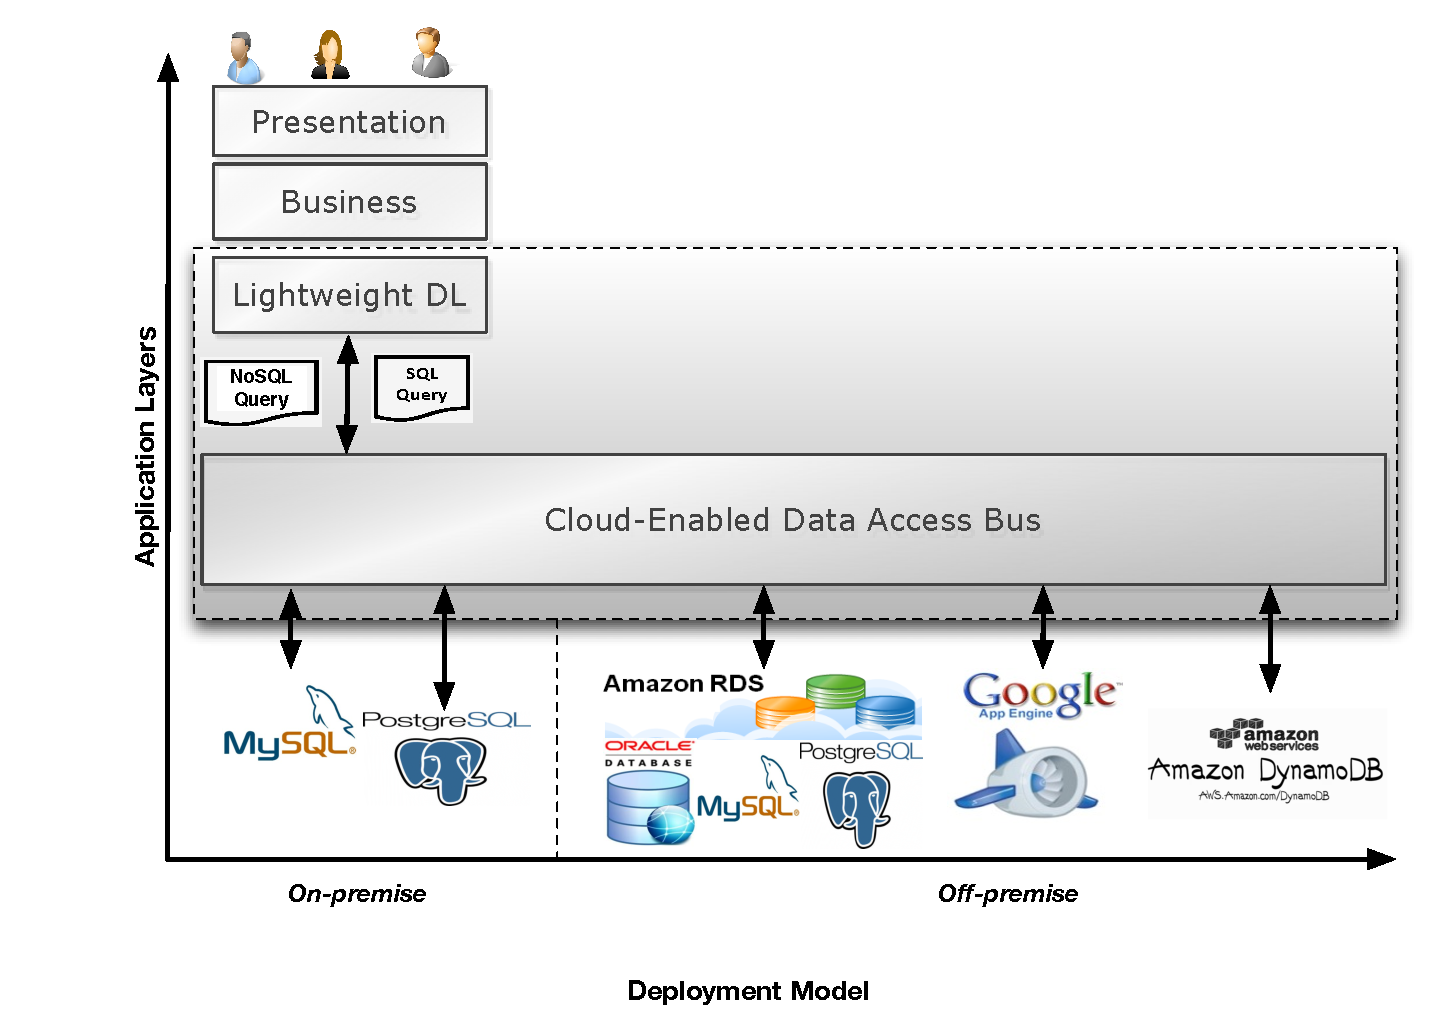
\includegraphics[width=0.925\textwidth, trim=0.0cm 0.0cm 0.0cm 0.0cm, clip]{./gfx/motivationScenario.pdf}
	\caption[Migration Scenario]{Migration Scenario to be filled }
	\label{fig:motivationscenario}
\end{figure}

As shown in Figure \ref{fig:motivationscenario}, the Cloud-Enabled Data Access bus provides access support between the hosted on-premise, and off-premise application's layers. Its main goal is to provide communication isolation between different applications and users, and maintain the transparency that the DL provided before the migration to the upper layers of the application's architecture. Support must be provided for two different databases types: MySQL and NoSQL databases, and between different providers. A tenant who migrates its data, e.g. to the Google SQL Datastore in Google App Engine, as shown in Figure \ref{fig:motivationscenario}, must be able to access his data with minimum adaptations of the components. Furthermore, storing or retrieving data whose storage is divided into multiple datasources requires a dynamic routing between backend data stores. Compatibility between different SQL and NoSQL databases must be also ensured. However, query and data transformation between different data sources types is out of the scope of this diploma thesis.  


\FloatBarrier